\subsection{Maximum Growth Rate is Determined by the Ribosomal Mass Fraction}
\label{sec:limit}
The 7 minute speed limit shown in \FIG{protein_synthesis}(B) assumes all
proteins in the cell are ribosomes. In order to connect this to the
experimental data (and physiological reality more broadly), we first need to relax this assumption and determine a
translation-limited growth rate. Here, we will assume that the cell is composed
of $N_\text{pep}$ peptide bonds and $R$ ribosomes, whose precise values will depend on the
growth rate $\lambda$. The protein subunits of each ribosomal protein sum to a
total of $\approx$ 7500 amino acids as noted earlier, which we denote by $L_R$.
With an average mass of an amino acid of $m_\text{AA} \approx$ 110
Da (BNID: 104877), the total ribosomal mass fraction  $\Phi_R$ is given by
\begin{equation}
  \Phi_R = \frac{m_\text{ribosomes} }{m_\text{proteome}} \approx \frac{m_\text{AA} \times R \times L_R}{m_\text{AA} \times N_\text{pep}} = \frac{R \times L_R}{N_\text{pep}}.
  \label{eq:phir}
\end{equation}
For exponentially growing cells \citep{godin2010}, the rate of cellular growth will
be related to the rate of protein synthesis via
\begin{equation}
  \lambda N_\text{pep} = r_t \times R \times f_a,
  \label{eq:lam_npep}
\end{equation}
where $r_t$ is the translation rate. Here, we've introduced a multiplicative
factor $f_a$ which represents the fraction of the ribosomes that are actively
translating. This term allows us to account for immature or
non-functional ribosomes or active sequestration of ribosomes through the action
of the secondary messenger alarmone (p)ppGpp in poorer nutrient conditions \cite{hauryliuk2015}.

Combining \EQ{phir} and \EQ{lam_npep} results in an expression for a
translation-limited growth rate, which is given by
\begin{equation}
\lambda_\text{translation-limited} = \frac{r_t\times \Phi_R\times f_a}{L_R}.
\label{eq:lam_limited}
\end{equation}
This result, derived in a similar manner in \cite{klumpp2013}, reflects
mass-balance under steady state growth and has long provided a rationalization
of the apparent linear increase in \textit{E. coli}'s ribosomal content as a
function growth rate \citep{goldberger1979, dennis2004, scott2010}. The
left-hand panel of \FIG{ribosome_limit}(A) shows this growth rate plotted as a
function of the ribosomal mass fraction.  In the regime where all ribosomes are
active ($f_a = 1$) and the entire proteome is composed of ribosomal proteins
($\Phi_R = 1$), indeed, we arrive at the maximum theoretical growth rate of $r_t
/ L_R$, and $\approx$ 7 min for \textit{E. coli}.

Connecting \EQ{lam_limited} to the proteomic data serving as the centerpiece of
our work, however, requires knowledge
of $f_a$ at each growth rate as proteomic measurements only provide a
measure of $\Phi_R$. Recently, \cite{dai2016} determined $f_a$ as a function of
the growth rate (\FIG{ribosome_limit}(A), right-hand panel, inset), revealing
that $f_a \approx 1$ at growth rates above 0.75 hr$^{-1}$ and $f_a < 1$ as the
growth rate slows. Using these data, we inferred the approximate active fraction
(see Appendix \nameref{sec:SI_f_a}) at each growth rate and used this to compute
$\Phi_R \times f_a$ (\FIG{ribosome_limit}(A), colored points in right-hand
panel). In general, these data skirt the translation-limited growth rate
determined using \EQ{lam_limited}, where we have taken $r_t$ to be the maximal elongation
rate of 17 amino acids per second measured by \cite{dai2016}. There is a notable
discrepancy between the data collected in \cite{schmidt2016, li2014} and that
collected from \cite{valgepea2013, peebo2015}. When compared to other
measurements (non-proteomic based) of the active ribosome mass fraction
(\FIG{ribosome_limit}(B), grey points in right-hand panel), the data from
\cite{valgepea2013} and \cite{peebo2015} are notably aberrant, suggesting a
systematic error in these data. These additional measurements come from a number
of recent studies and are determined from measurements of total RNA to total
protein mass ratios (\FIGSUPP[ribosome_limit]{ribosome_limit_supp}).

Together, these results illustrate that the growth rates observed across the
amalgamated data sets are close to the translation-limited growth rate
determined through  ribosomal activity, at least for the data reported in
\cite{schmidt2016} and \cite{li2014}. While this is a useful framework to
consider how the relative abundance of ribosomes (compared to all other
proteins) defines the growth rate, it is worth noting that as growth rate
increases, so does the cell size and therefore so will the total proteomic mass
\citep{basan2015}. With a handle on how elongation rate and the total number of
peptide bonds per proteome is related to the growth rate, we now expand this
description to account for the increasing cell size and ribosome copy number at
faster growth rates,  enabling us to identify a potential bottleneck in the
synthesis of rRNA.

\begin{figure}
  \begin{fullwidth}
        \centering{
        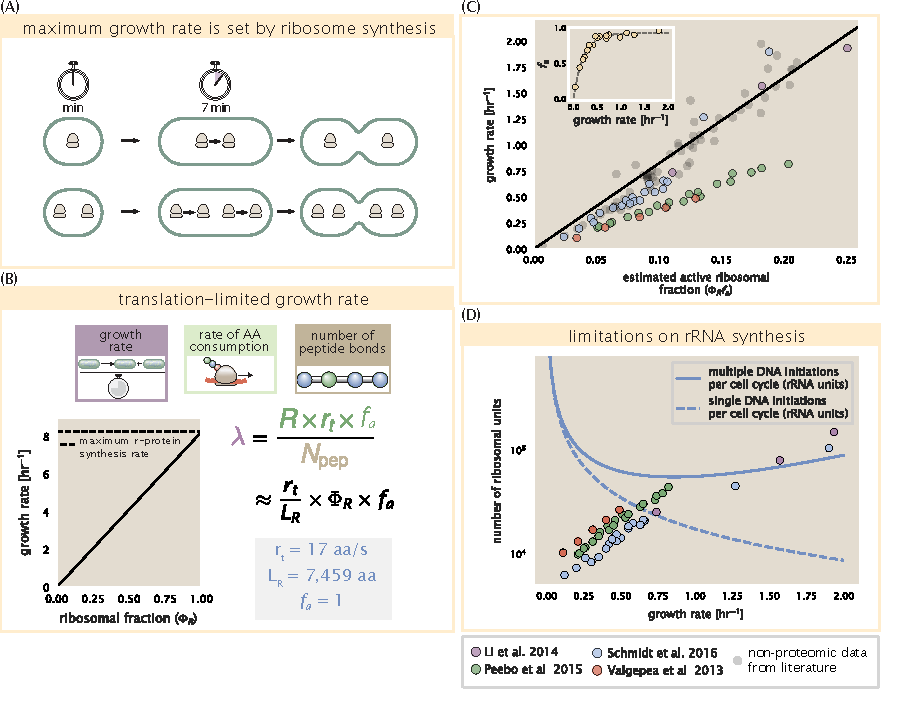
\includegraphics{main_figs/fig7_ribosome_as_limit.pdf}
        \caption{\textbf{Translation-limited growth rate.}  (A) \textit{left}:
        Translation-limited growth as a function of the ribosomal fraction. The
        solid line is calculated for an elongation rate of 17 aa per second.
        The dashed line corresponds to the maximum rate of ribosomal protein
        synthesis ($\approx$ 7 min).
        \textit{right}: Translation-limited growth rate as a function of the actively translating ribosomal fraction.
        The actively translating ribosomal fraction is calculated using the
        estimated values of $f_a$ from  \cite{dai2016} (shown in inset; see
        Appendix \nameref{sec:SI_f_a} for additional detail). Gray data points
        show additional measurements from literature and consider further in
        the supplemental figure part (A).
        (B) Maximum number of
        rRNA units that can be synthesized as a function of growth rate.
        Solid curve corresponding to the rRNA copy number is calculated by
        multipyling the number of rRNA operons by the estimated number of
        $\langle\text{\# ori}\rangle$ at each growth rate. The quantity
        $\langle\text{\# ori}\rangle$ was calculated using Equation 4 and
        the measurements from \cite{si2017}. The dashed line shows the maximal
        number of functional rRNA units produced from a single chromosomal
        initiation per cell cycle. } \label{fig:ribosome_limit}


        \figsupp[Comparison of $\Phi_R f_a$ with literature and estimation of
        $\langle$\# ori$\rangle$.]{(A) Actively translating ribosomal
        fraction versus growth rate. The actively translating ribosomal
        fraction is calculated using the estimated values of $f_a$ from
        \cite{dai2016} (shown in inset; see Appendix \nameref{sec:SI_f_a} for
        additional detail). Additional measurements in addition to the
        proteomic measurements are based on measurements of cellular RNA to
        protein ratio, with $\Phi_R \approx$ the cellular RNA to protein
        ratio divided by 2.1 \citep{dai2016}. (B) Experimental measurements
        of the cell doubling time $\tau$ and cell cycle time $t_{cyc}$ from
        Si \textit{et al.} (2017). Dashed line shows fit to the data, which
        were used to estimate $\langle$\# ori$\rangle$. $t_{cyc}$ was assumed
        to vary in proportion to $\tau$ for doubling times greater than 40
        minutes, and reach a minimum value of 73 minutes. See Appendix
        \nameref{sec:SI_ori} for additional details exact estimation of rRNA
        copy number. Red data points correspond to measurements in strain
        MG1655, while light green points are for strain NCM3722. Schematic
        shows the expected increase in replication forks (or number of ori
        regions) as \textit{E. coli} cells grow faster.
        }{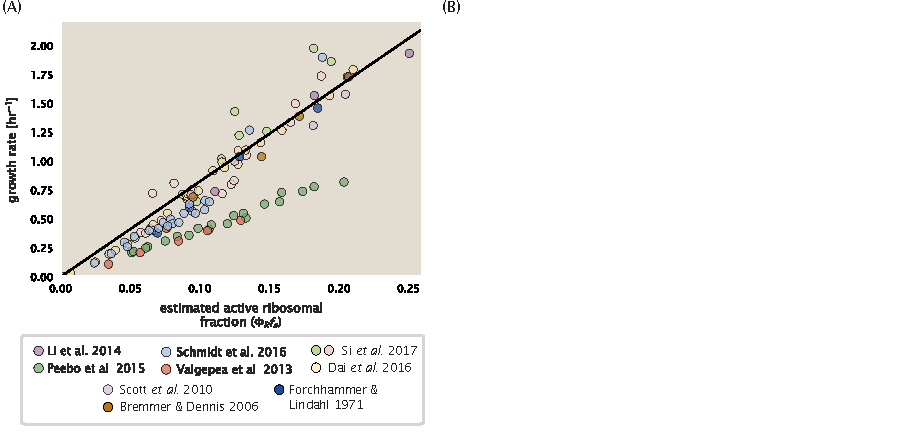
\includegraphics{main_figs/fig7_ribosome_as_limit_Supp.pdf}}\label{figsupp:ribosome_limit_supp}
        }
  \end{fullwidth}
\end{figure}

\subsection{rRNA Synthesis Presents a Potential Bottleneck During Rapid Growth}
Even under idealized experimental conditions, \textit{E. coli} rarely
exhibits growth rates above 2 hr$^{-1}$ \citep{bremer2008}, which is still
well-below the synthesis rate of a single ribosome, and below the maximum
growth rates reported for several other bacteria \citep{roller2016}. While we
have considered potential limits imposed by translation of ribosomal
\textit{proteins}, here we consider potential limiting regimes specific to the
synthesis of rRNA.

Due to multiple initiations of chromosomal replication per cell doubling, the
effective number of rRNA operons increases with growth rate and will do so in
proportion to the average number of origins per cell, $\langle$\# ori$\rangle$.
This later parameter is set by how often replication must be initiated in order
to keep up with cell doubling times $\tau$, whose time may be shorter than the
cell cycle time $\tau_{cyc}$ (referring to the time from replication initiation to
cell division) \citep{dennis2004}. This is quantified by
\begin{equation}
    \langle \text{\# ori} \rangle = 2^{\tau_{cyc} / \tau} = 2^{\tau_{cyc} \lambda / \log(2)}.
    \label{eq:Nori}
\end{equation}
We used the experimental measurements of $\tau_{cyc}$ (the timescale of
chromosome replication and cell division) and $\tau$ (the timescale of a cell
doubling) from
\cite{si2017} (\FIGSUPP[ribosome_limit]{ribosome_limit_supp}(B)) to calculate
$\langle$\# ori$\rangle$  with \EQ{Nori} as a function of growth rates. For
growth rates above about 0.5 hr$^{-1}$, $t_{cyc}$ is approximately constant at
about 70 minutes, implying that $\langle$\# ori$\rangle$ will grow
exponentially with growth rates beyond 0.5 hr$^{-1}$. As the rRNA operons are predominantly located
close to origin of replication (BNID: 100352), we make the simplifying
assumption that that the number of rRNA operons  will be directly proportional
to $\langle$\# ori$\rangle$.

Returning to our rule-of-thumb of 1 functional rRNA unit per second per
transcribing operon, we estimate the maximum number of ribosomes that could be
made as a function of growth rate (\FIG{ribosome_limit}(B), blue curve).
Although we expect this estimate to significantly overestimate rRNA abundance at
slower growth rates ($\lambda < 0.5\, \text{hr}^{-1}$), this provides a useful
reference alongside the proteomic measurements, particularly in the regime of
fast growth. For growth rates above about 1 hr$^{-1}$, for example, we find that
cells will need to transcribe rRNA near their maximal rate. As a counter
example, if \textit{E. coli} did not initiate multiple rounds of replication,
but manged to replicate their chromosome within the requisite time limit, they
would be unable to make enough rRNA for the observed number of ribosomes (dashed
blue curve in \FIG{ribosome_limit}(C)). The convergence between the maximum rRNA
production and measured ribosome copy number suggests rRNA synthesis may begin
to present a bottleneck at the fastest growth rates due to the still-limited
copies of rRNA genes.


% It is now well-documented that \textit{E. coli} cells add a constant volume per
% origin of replication, which is robust to a remarkable array of cellular
% perturbations \citep{si2017}.

% To consider
% this  in the context of the proteomic data, we used measurements of $\tau_{cyc}$
% and  $\tau$ from \cite{si2017} (\FIG{translation_ecoli_partA}(A)) to
% calculate $\langle$\# ori$\rangle$  with \EQ{Nori} at different growth
% rates. For ribosomal synthesis, we find an approximately linear correlation
% between ribosome copy number and $\langle$\# ori$\rangle$
% (\FIG{translation_ecoli_partA}(B)).
%
% For a constant cell cycle time, which is observed at growth rates above about
% 0.5 hr$^{-1}$ (\FIG{translation_ecoli_partA}(A), \citep{helmstetter1968}),
% \EQ{Nori} states that $\langle \text{\# ori} \rangle$ will need to increase
% exponentially with the growth rate.

% speak in  mor
% We begin by considering the length of time needed to replicate a single
% ribosome. As mentioned in our discussion of rRNA synthesis, the bacterial
% ribosome is approximately 2/3 RNA by mass, with the remaining 1/3 being composed
% of protein. Of the $\approx$ 50 ribosomal subunits, all are present as a single
% copy save for RplL which is present in four copies. Taking these proteins
% together, a single ribosome is composed of $L_R \approx$ 7500 individual amino
% acids, approximately equal to the number of peptide bonds. Again assuming a
% reasonable translation rate of $r_t \approx$ 15 amino acids per second, we arrive at
% an simple estimate that it takes on the order of  $L_R / r_t \approx$ 7 minutes to
% translate a single ribosome.
% However, we can consider the translation limited growth rate as a function of
% the fraction $\Phi_R$ of the total number of amino acids in the proteome $N_\text{pep}$
% that are sequestered in a ribosome, $N_\text{pep}^\text{(ribosome)}$. To compute this quantity, we
% note that the number of amino acids in a ribosome is related to the protein mass
% via
% \begin{equation}
%   m_\text{ribosome} \approx L_R \times m_\text{AA}
%   \label{eq:mribo}
% \end{equation}
% where $m_\text{AA}$ is the average mass of an amino acid which is $\approx$ 110
% Da (BNID: 104877). Similarly, we can compute the mass of the total cellular
% proteome as
% \begin{equation}
%   m_\text{proteome} \approx N_\text{pep} \times m_\text{AA}.
%   \label{eq:mproteome}
% \end{equation}

% Together, \EQ{mribo} and \EQ{mproteome} allow us to define the ribosomal mass
% fraction as
% \begin{equation}
%   \Phi_R = \frac{m_\text{ribosome} \times R}{m_\text{proteome}} \approx \frac{R \times L_R}{N_\text{pep}}.
%   \label{eq:phir}
% \end{equation}
% Relating the number of peptide bonds to be synthesized to complete division to
% the number of ribosomes per cell in this manner allows us to enumerate an
% expression for translation-limited growth. As cells grow exponentially in time
% \cite{godin2010}, the rate of cellular growth can be computed as
% \begin{equation}
% N_\text{pep} \lambda = r_t \times R \times f_a,
% \label{eq:exp_cell_growth}
% \end{equation}
% where $\lambda$ is the cellular growth rate and $f_a$ is a multiplicative factor
% which describes the fraction of ribosomes actively translating. This latter term
% allows us to account for the possibility of nonfunctional, immature ribosomes or
% active sequestration of ribosomes through small-molecule alarmones such as
% (p)ppGpp which can be significant at slow growth rates \citep{dennis2004,
% dai2016}. Combining \EQ{phir} and \EQ{exp_cell_growth} yields an expression for
% the translation limited growth rate
% \begin{equation}
% \lambda_\text{translation-limited} \approx \frac{r_t}{L_R}\Phi_Rf_a.
% \label{eq:lam_lim}
% \end{equation}

% This expression is plotted in the top panel of \FIG{limit}(B) assuming $f_a =
% 1$. When $\Phi_R \approx 1$ (i.e. when all proteins in the cell are ribosomal),
% the maximum growth rate corresponds to the speed limit of $\approx$ 7 min,
% illustrated by a dashed line in the top panel of \FIG{limit}(B). As the product
% $f_a \times \Phi_R$ is
% decreased, meaning the ribosomes occupy a smaller and smaller proportion of the
% proteome, we observe that the growth similarly decreases. To make a connection
% with the proteomic data, we require a means to estimate $f_a$ at each growth
% rate. Recent measurements by \cite{dai2016} reveal that $f_a \approx 1$ at fast
% growth rates ($>$ 0.75 hr$^{-1}$) and monotonically decreases as slower growth
% rates (\FIG{limit} (B), inset in bottom plot). Using these data, we estimated
% $f_a$ for each growth rate present in the proteomic data set. In general, these
% data appear to skirt this translation limited growth regime as growth conditions
% change (\FIG{limit}(B), colored points in bottom plot). There is a notable
% discrepancy between the data collected in \cite{schmidt2016, li2014} and that
% collected from \cite{valgepea2013, peebo2015}. When compared to other,
% non-proteomic wide measurements of the active ribosome mass fraction
% (\FIG{limit} (B), grey points in bottom plot), the data from \cite{valgepea2013}
% and \cite{peebo2015} are notably aberrant, suggesting a systematic error in
% these data.


% To  gain some intuition into how ribosomal synthesis influences
% bacterial growth, we again consider the total number of peptide bonds that must
% be synthesized, which we denote as $N_\text{pep}$. With cells growing exponentially in time
% \citep{godin2010}, the rate of cellular growth will be related to the rate of protein synthesis by
% \begin{equation}
%     N_\text{pep} \lambda = r_t R f_a,
%     \label{eq:mass_balance}
% \end{equation}
% where $\lambda$ is the cell growth rate,  $r_t$ is the maximum
% elongation rate in AA per second, and $R$ is the average ribosome copy
% number per cell. The multiplicative factor $f_a$ refers to the fraction of
% ribosomes actively translating, and allows us to account for the possibility of
% nonfunctional, immature ribosomes or active sequestration of ribosomes, mediated
% by the secondary-messenger molecule alarmones, such as guanosine pentaphosphate
% [(p)ppGpp] at slow growth \citep{dennis2004, dai2016}.

% Rather than speaking in terms of absolute ribosome abundance, we can account for
% the ribosome content as was defined by \cite{scott2010} as the mass of fraction
% of the proteome occupied by ribosomes $\Phi_R$. Similarly, as $N_\text{pep}$ is related to
% the total protein mass through the molecular weight of each protein, we can also consider the growth
% rate in terms of the fraction of the total proteome mass dedicated to ribosomal
% proteins. By making the approximation that an average amino acid has a molecular
% weight of 110 Da (BNID: 104877), the total protein mass $m_\text{protein}$ is
% related to $N_\text{pep}$ by $(m_\text{protein}/\text{110 Da}) \times N_A$,
% where $N_A$ is Avogadro's number. Similarly, $R$ is related to the ribosomal
% protein mass by $R \approx (m_R/\text{800 Da}) \times N_A$, where 800 Da
% reflects the summed molecular weight of all ribosomal subunits.  This allows us
% to approximate  $R / N_\text{pep} \approx \Phi_R / L_R$,  where $\Phi_R$ is the
% ribosomal mass fraction $m_\text{protein}/m_R$, and $L_R$ the ratio of 800 kDa /
% 110 Da per amino acid or, alternatively, the total length in amino acids that
% make up a ribosome. Under this parameterization, the translation-limited growth rate can then be written in
% the form
% \begin{equation}
% \lambda_{\textrm{translation-limited}} \approx \frac{r_t}{L_R}  \Phi_R f_a.
% \label{eq:translation_limit_growth_rate}
% \end{equation}
% This is plotted as a function of the ribosomal fraction $\Phi_R$ in the top panel of
% \FIG{ribosome_limit}(A), where we take $L_R \approx$ 7500 AA, corresponding to
% the length in amino acids for all ribosomal subunits of the 50S and 30S complex
% (BNID: 101175), and $f_a$ = 1. To compare this relationship to the proteomic
% data, we make use of recent measurements of $f_a$ from \cite{dai2016}
% (\FIG{ribosome_limit}(A), bottom inset) to estimate the active
% fraction of ribosomal protein across each proteomic data set
% (\FIG{ribosome_limit}(A), colored points, bottom). In general, the data appear to
% skirt this limit in growth rate as nutrient conditions vary. There is a notable discrepancy
% in the data from \cite{peebo2015, valgepea2013}, where cells appear to grow
% substantially slower given their estimated ribosomal fraction. Here we have
% also collected a number of recent non-proteomic measurements of ribosomal fraction and
% find them most consistent with the measurements from \cite{li2014,
% schmidt2016} (gray points; also see \FIGSUPP[ribosome_limit]{ribosome_limit_supp}(A)).

% The growth rate defined by \EQ{translation_limit_growth_rate} reflects
% mass-balance under steady state growth and has long provided a rationalization
% of the apparent linear increase in \textit{E. coli}'s ribosomal content as a
% function of growth rate \citep{goldberger1979, scott2010}. The maximum rate,
% when $\Phi_R$ = 1, could only be achieved if a cell contained only ribosomes \citep{dill2011}.
% This corresponds to the synthesis time of all ribosomal subunits, $L_R/ r_t
% \approx$ 7 minutes and interestingly, is independent of the
% absolute number of ribosomes (\FIG{ribosome_limit}(B)). To return to our earlier comments on
% parallelization, it is this step that is rate-limiting, with each ribosome being
% required to produce a second ribosome. Unless elongation rate increased, or
% cells could trim their total ribosomal protein mass, this dependency limits both
% the maximum growth rate (when $\Phi_R$ = 1), and also the achieveable growth
% rate under more moderate values of $\Phi_R$.
